% Petri net "Producer/consumer", generated by pnm
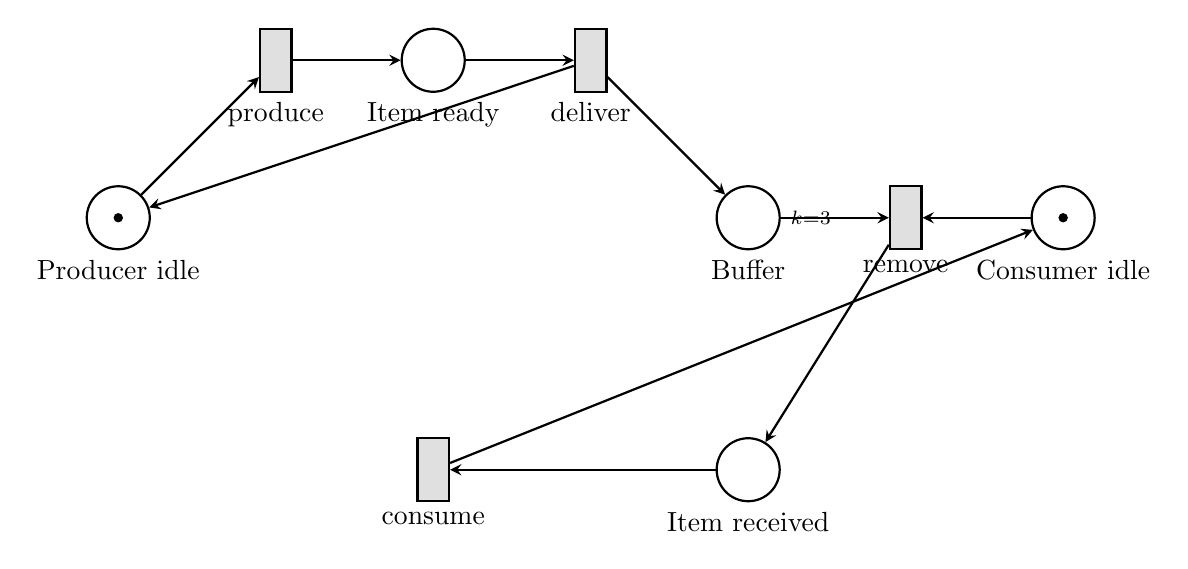
\begin{tikzpicture}
  \tikzset{
    place/.style={circle, draw=black, fill=white, thick, minimum size=8mm, inner sep=0pt},
    transition/.style={rectangle, draw=black, fill=black!12, thick, minimum width=4mm, minimum height=8mm, inner sep=0pt},
    arc/.style={->, >=stealth, thick},
    token/.style={circle, fill=black, inner sep=1.2pt},
  }
  % Places
  \node[place, label={below:{Producer idle}}] (prod_idle) at (0,3.2) {};
  \node[place, label={below:{Item ready}}] (prod_ready) at (4,5.2) {};
  \node[place, label={below:{Buffer}}, label={[font=\scriptsize]right:{$k{=}3$}}] (buffer) at (8,3.2) {};
  \node[place, label={below:{Consumer idle}}] (cons_idle) at (12,3.2) {};
  \node[place, label={below:{Item received}}] (cons_ready) at (8,0) {};
  \node[token] at (0,3.2) {};
  \node[token] at (12,3.2) {};
  % Transitions
  \node[transition, label={below:{produce}}] (produce) at (2,5.2) {};
  \node[transition, label={below:{deliver}}] (deliver) at (6,5.2) {};
  \node[transition, label={below:{remove}}] (remove) at (10,3.2) {};
  \node[transition, label={below:{consume}}] (consume) at (4,0) {};
  % Arcs
  \draw[arc] (prod_idle) -- (produce);
  \draw[arc] (produce) -- (prod_ready);
  \draw[arc] (prod_ready) -- (deliver);
  \draw[arc] (deliver) -- (prod_idle);
  \draw[arc] (deliver) -- (buffer);
  \draw[arc] (buffer) -- (remove);
  \draw[arc] (cons_idle) -- (remove);
  \draw[arc] (remove) -- (cons_ready);
  \draw[arc] (cons_ready) -- (consume);
  \draw[arc] (consume) -- (cons_idle);
\end{tikzpicture}
